\documentclass[8pt]{beamer}
\usepackage{geometry}
\usepackage{amsmath}
\usepackage{amsfonts}
\usepackage{amssymb}
\usepackage{enumerate} 
\usepackage{amsthm}
\usepackage{graphicx}
\usepackage{indentfirst}
\usepackage{subfig}
\usepackage{booktabs}
\usepackage{multirow}
%\usepackage{array}
%\usepackage{tikz}

\newtheorem{thm}{Theorem}[section]
\newtheorem{defi}{Definition}[section]
\numberwithin{equation}{section}
%\def\layersep{1.5cm}

\mode<presentation> {

% The Beamer class comes with a number of default slide themes
% which change the colors and layouts of slides. Below this is a list
% of all the themes, uncomment each in turn to see what they look like.

%\usetheme{default}
%\usetheme{AnnArbor}
%\usetheme{Antibes}
%\usetheme{Bergen}
%\usetheme{Berkeley}
\usetheme{Berlin}
%\usetheme{Boadilla}
%\usetheme{CambridgeUS}
%\usetheme{Copenhagen}
%\usetheme{Darmstadt}
%\usetheme{Dresden}
%\usetheme{Frankfurt}
%\usetheme{Goettingen}
%\usetheme{Hannover}
%\usetheme{Ilmenau}
%\usetheme{JuanLesPins}
%\usetheme{Luebeck}
%\usetheme{Madrid}
%\usetheme{Malmoe}
%\usetheme{Marburg}
%\usetheme{Montpellier}
%\usetheme{PaloAlto}
%\usetheme{Pittsburgh}
%\usetheme{Rochester}
%\usetheme{Singapore}
%\usetheme{Szeged}
%\usetheme{Warsaw}

% As well as themes, the Beamer class has a number of color themes
% for any slide theme. Uncomment each of these in turn to see how it
% changes the colors of your current slide theme.

%\usecolortheme{albatross}
%\usecolortheme{beaver}
%\usecolortheme{beetle}
%\usecolortheme{crane}
%\usecolortheme{dolphin}
%\usecolortheme{dove}
%\usecolortheme{fly}
%\usecolortheme{lily}
%\usecolortheme{orchid}
%\usecolortheme{rose}
%\usecolortheme{seagull}
%\usecolortheme{seahorse}
\usecolortheme{whale}
%\usecolortheme{wolverine}

%\setbeamertemplate{headline}{  \leavevmode%
%  \begin{beamercolorbox}[wd=.5\paperwidth,ht=2.5ex,dp=1.125ex]{section in head/foot}%
%    \hbox to 0.55\paperwidth{\insertsectionhead\hfil}
%  \end{beamercolorbox}%
%  \begin{beamercolorbox}[wd=.5\paperwidth,ht=2.5ex,dp=1.125ex]{subsection in head/foot}%
%    \hbox to 0.55\paperwidth{\insertsubsectionhead\hfil}
%  \end{beamercolorbox}%
%}

\setbeamertemplate{headline}
{
   \leavevmode%
   \hbox{%
   \begin{beamercolorbox}[wd=.5\paperwidth,ht=2.25ex,dp=1ex,right]{section in head/foot}%
     \usebeamerfont{section in head/foot}\insertsectionhead\hspace*{3ex}
   \end{beamercolorbox}%
   \begin{beamercolorbox}[wd=.5\paperwidth,ht=2.25ex,dp=1ex,left]{subsection in head/foot}%
     \usebeamerfont{subsection in head/foot}\hspace*{3ex}\insertsubsectionhead
   \end{beamercolorbox}}%
   \vskip0pt%
}

%\setbeamertemplate{footline} % To remove the footer line in all slides uncomment this line
%\setbeamertemplate{footline}{%
%   \usebeamercolor[fg]{page number in head/foot}%
%   \usebeamerfont{page number in head/foot}%
%   \hspace{1em}\insertshortauthor\hfill%
%   \insertpagenumber\,/\,\insertpresentationendpage\kern1em\vskip2pt%
%} % To replace the footer line in all slides with a simple slide count uncomment this line

\setbeamertemplate{navigation symbols}{} % To remove the navigation symbols from the bottom of all slides uncomment this line
}

\title{Pricing Asian Options on Commodities with GARCH Model}
\author{Lue Shen\textsuperscript{1}, Leheng Chen\textsuperscript{1}, Chu Song\textsuperscript{1} and Jing Qian\textsuperscript{1}} % Authors
\institute{\textsuperscript{1}Department of Mathematics, the Hong Kong University of Science and Technology, Hong Kong SAR, China} % Institution 1


%\institute{SYSU}
\date{May 15th, 2019}

\begin{document}
\begin{frame}
\titlepage % Print the title page as the first slide
\end{frame}

\begin{frame}
\frametitle{Contents}
\tableofcontents
\end{frame}

\section{Introduction}

\frame{\tableofcontents[currentsection]}

\subsection{Commodities, Commodity Futures and Asian Options}
\begin{frame}{Commodities, Commodity Futures and Asian Options}
\begin{itemize}
	\item Commodities: basic good used in commerce that is interchangeable with other commodities of the same type.
	\item Commodity Futures: agreements to buy or sell a raw material at a specific date in the future at a particular price.
	\begin{equation}
	F_t = S_t - f_t
	\end{equation}
	\item Asian Options: average value options, an exotic option whose payoff is determined by the average underlying price over some pre-set period of time. This averaging feature provides
	\begin{itemize}
		\item Risk reduction of market manipulation of the underlying instrument close to maturity \cite{kemna1990pricing}.
		\item Lower cost than European or American options with same strike and maturity.
	\end{itemize}

	\begin{equation} \label{eq:1}
	\begin{aligned}
	C_T &= (A_T(t,T) - K)^+
	\\
	P_T &= (K - A_T(t,T))^+
	\\
	A_T(0,T) &= \frac 1T \sum_{t=0}^T S_t = \frac 1T \int_0^T S_t dt
	\\
	\tilde{A}_T(0, T) &= (\prod_{t=0}^T S_t )^{\frac 1T} = \exp (\frac 1T \int_0^T \log S_t dt)
	\end{aligned}
	\end{equation}
	
\end{itemize}

\end{frame}

\subsection{Prevailing Pricing Methods}
\begin{frame}{Prevailing Pricing Methods}
\begin{itemize}
\item Semi-Analytical: fast Fourier transform (FFT) and convolutions \cite{carverhill1990average} \cite{benhamou2000fast}.
\item Approximation: approximate the real distribution of the average underlying price at the maturity with tractable ones, such as Edgeworth series expansion \cite{turnbull1991quick} or lognormal distributions \cite{levy1992pricing}.
\item Monte Carlo: combination of stochastic models and Monte Carlo simulations \cite{kemna1990pricing}.
\end{itemize}
\end{frame}


\subsection{Proposed Methods}
\begin{frame}{Proposed Methods}
\begin{itemize}
\item GARCH model: Monte Carlo simulations with GJR-GARCH model.
\item Non-GARCH models: binomial tree model and Monte Carlo simulations with constant volatility.
\item Model comparison criteria: ARE criteria \cite{zhu2015model}.

\begin{equation}
ARE = \frac{1}{N} \sum^N_{j = 1} \frac{\vert V^{model}_j - V^{market}_j \vert}{V^{market}_j} \times 100
\end{equation}

\end{itemize}
\end{frame}

\section{Time Series Data}

\frame{\tableofcontents[currentsection]}

\subsection{Commodities}
\begin{frame}{Commodities}
16 commodities from 3 broad categories are selected for analysis. For each of them, price data of the most liquid/major future contract is collected for analysis.

\textbf{Energy:}
\begin{itemize}
	\item Crude Oil: WTI Financial Futures
	\item Natural Gas: Henry Hub Natural Gas Futures
	\item Refined Products: RBOB Gasonline Futures
	\item Biofuels: Chicago Ethanol (Platts) Futures
	\item Coal: Coal (API2) CIF ARA (ARGUS-McCloskey) Futures
\end{itemize}

\textbf{Agriculture:}
\begin{itemize}
	\item Corns: Corns Futures
	\item Wheats: Chicago SRW Wheat Futures
	\item Soybean: Soybean Futures
	\item Soybean Meal: Soybean Meal Futures
	\item Soybean Oil: Soybean Oil Futures
	\item Livestock: Live Cattle Futures
	\item Livestock: Lean Hog Futures
\end{itemize}

\textbf{Metals:}
\begin{itemize}
	\item Gold: Gold Futures
	\item Silver: Silver Futures
	\item Platinum: Platinum Futures
	\item Copper: Copper Futures
\end{itemize}
\end{frame}

\subsection{Asian Options}
\begin{frame}{Asian Options}
Strike prices and maturities from 5 commodity option contracts are collected to construct numerical examples for proposed pricing models. There are 319 option contracts (call put pairs) in total, with maturity varying from 5 days to 5 years. Their contract specifications and settlement prices are collected as reference. 

Here is the list:

\begin{itemize}
	\item WTI Crude Oil Asian Option
	\item Chicago Ethanol (Platts) Asian Option
	\item Gold American Option
	\item Silver American Option
	\item Natural Gas European Option
\end{itemize}
\end{frame}

\subsection{Data Source}
\begin{frame}{Data Source}
\begin{itemize}
	\item Commodity future prices: investing.com, with time span from 2000-01-03 to 2019-03-22, and there are 16 price time series in total.
	\item Commodity options: recorded manually from CME group website, and there are 319*2=638 options in total (319 call put pairs).
	\item Risk free interest rates: US treasury yield curve on 2019-03-22 from US government website.
\end{itemize}
\end{frame}

\subsection{Data Preprocess}
\begin{frame}{Data Preprocess}
Two major preprocessing steps:

\begin{itemize}
	\item Time series concatenation: concat price series into one data table with respect to dates.
	\item Convert risk free spot curve to forward curve:
	
	\begin{equation} \label{eq:4}
	\begin{aligned}
	f(t_i, t_{i+1}) &= \frac {\log (e^{r_{t_{i+1}}t_{i+1}} / e^ {r_{t_i}t_i)}} {t_{i+1} - t_i}
	\\
	&= \frac {r_{t_{i+1}}t_{i+1} - r_{t_i}t_i}{t_{i+1} - t_i}
	\end{aligned}
	\end{equation}
\end{itemize}

Missing value preprocessing:

\begin{itemize}
	\item Time series analysis: for two time series selected for correlation analysis, all the date points with missing values will be removed.
	\item Pricing: date points with missing values will be dropped.
\end{itemize}
\end{frame}

\subsection{Correlation Analysis}
\begin{frame}{Correlation Analysis}
Correlation analysis is a method of statistical evaluation used to study the strength of a relationship between two, numerically measured, continuous variables. In this step, the correlation coefficients among future prices and price log returns are calculated respectively by equation \ref{eq:correlation}.

\begin{equation} \label{eq:correlation}
\begin{aligned}
\rho_{xy} &= \frac {\sum_{i=1}^n (x_i-\bar x)(y_i-\bar y)}{(n-1)s_xs_y}
\\
&=\frac {\sum_{i=1}^n (x_i-\bar x)(y_i-\bar y)}{\sqrt{\sum_{i=1}^n(x_i - \bar x)^2 \sum_{i=1}^n(y_i - \bar y)^2}}
\end{aligned}
\end{equation}

Findings from heat maps:

\begin{itemize}
	\item Price correlations: 
		\begin{itemize}
			\item Many strong positive linear relationships.
			\item Few commodities are less correlated to all other commodities.
			\item Randomness of correlations in commodity prices.
		\end{itemize}
	\item Log return correlations: strong (positive) correlations are only presented between commodities within the same category, especially in agriculture or metals.
	
\end{itemize}
\end{frame}

\begin{frame}{Correlation Analysis}
\begin{figure}[!ht]
	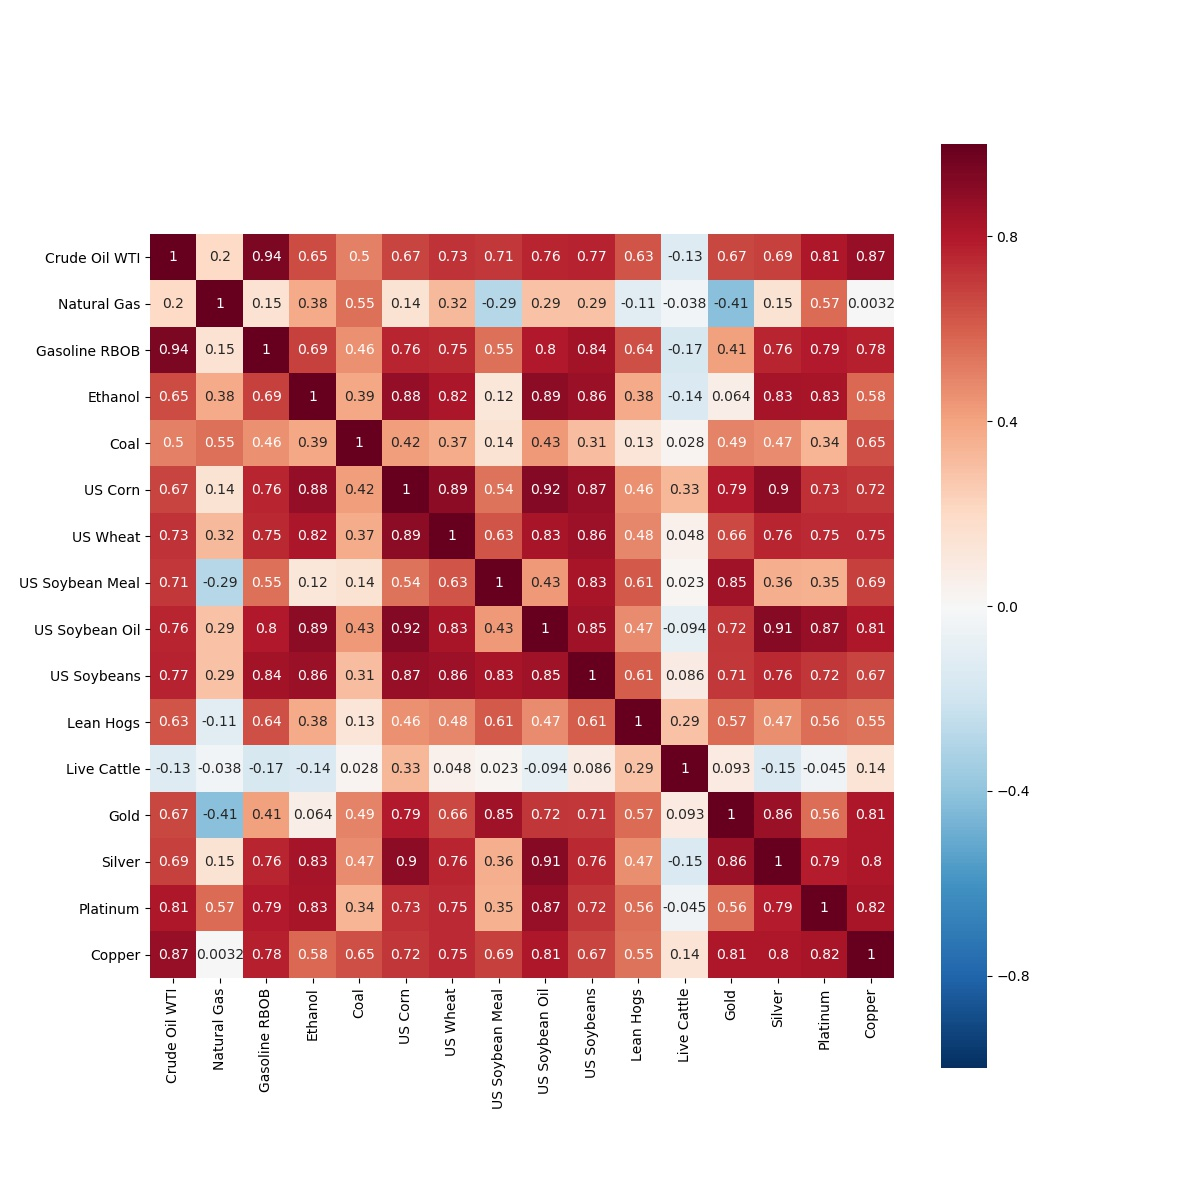
\includegraphics[width=7cm]{priceCorrelation.jpg} % Figure image
	\caption{Correlation Analysis of Commodity Prices} % Figure caption
	\label{priceCorrelation} % Label for referencing with \ref{bear}
\end{figure}

\end{frame}

\begin{frame}{Correlation Analysis}

\begin{figure} [!ht]
	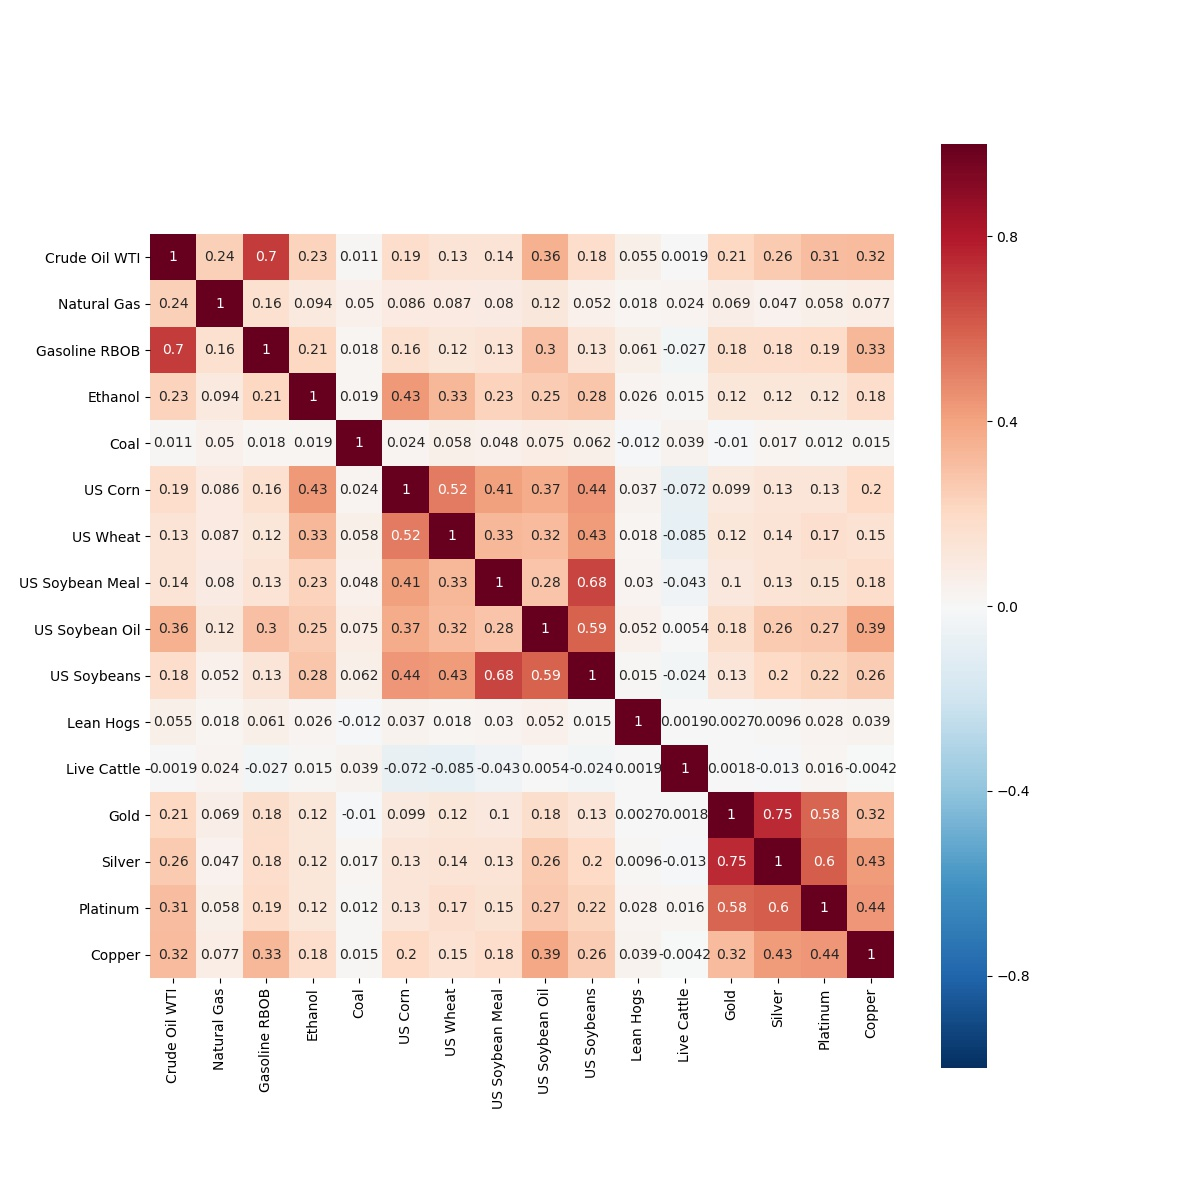
\includegraphics[width=7cm]{logRtCorrelation.jpg} % Figure image
	\caption{Correlation Analysis of Commodity Log Returns} % Figure caption
	\label{logRtCorrelation} % Label for referencing with \ref{bear}
\end{figure}
\end{frame}

\section{Pricing Models}

\frame{\tableofcontents[currentsection]}

\subsection{Monte Carlo GJR-GARCH Model}

\begin{frame}{GJR-GARCH Model}
The Glosten-Jagannathan-Runkle GARCH (GJR-GARCH) model by Glosten, Jagannathan and Runkle (1993) models asymmetry in the ARCH process.

For $GJR-GARCH(p, o, q)$, the model is expressed as the following:

\begin{equation}
\begin{aligned}
r_t &= \log S_t - \log S_{t-1}
\\
r_t &= \mu +\epsilon_t
\\
\epsilon_t &= \sigma_t Z_t
\\
\sigma_t^2 &= \omega + \sum_{i=1}^p {\alpha_i \epsilon_{t-i}^2} + \sum_{j=1}^o {\gamma_j \epsilon_{t-j}^2 I_{\epsilon_{t-j} < 0}} + \sum_{k=1}^q {\beta_k \sigma_{t-k}^2}
\end{aligned}
\end{equation}

This model will be used to fit the historical log returns and predict the mean volatility along the simulated Monte Carlo path, since

\begin{equation}
\sigma_0(t) = E_0[\sigma(t)]
\end{equation}

\end{frame}

\begin{frame}{GJR-GARCH Model Volatility Predictions}

\begin{figure}[!ht]
	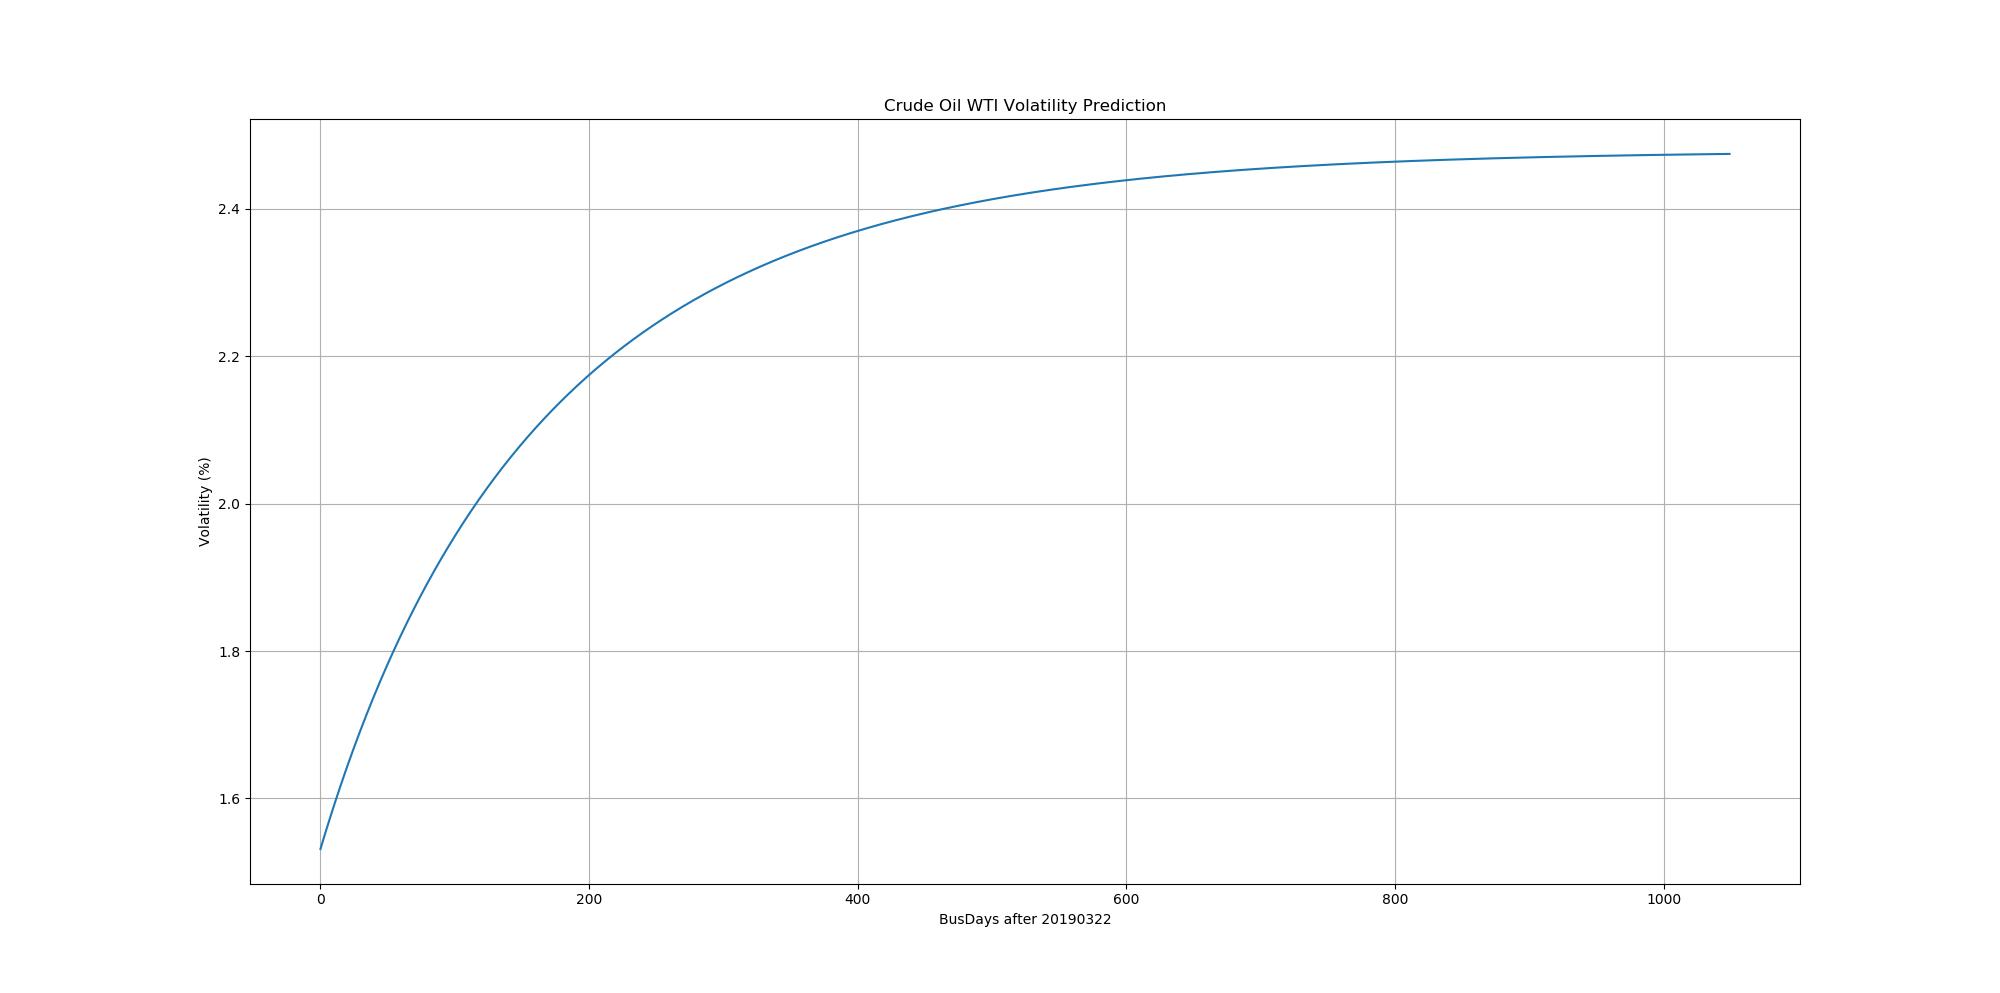
\includegraphics[width=\linewidth]{CrudeOilvol.png} % Figure image
	\caption{Volatility Prediction on Crude Oil} % Figure caption
	\label{oil pred} % Label for referencing with \ref{bear}
\end{figure}

\end{frame}

\begin{frame}{GJR-GARCH Model Volatility Predictions}

\begin{figure}[!ht]
	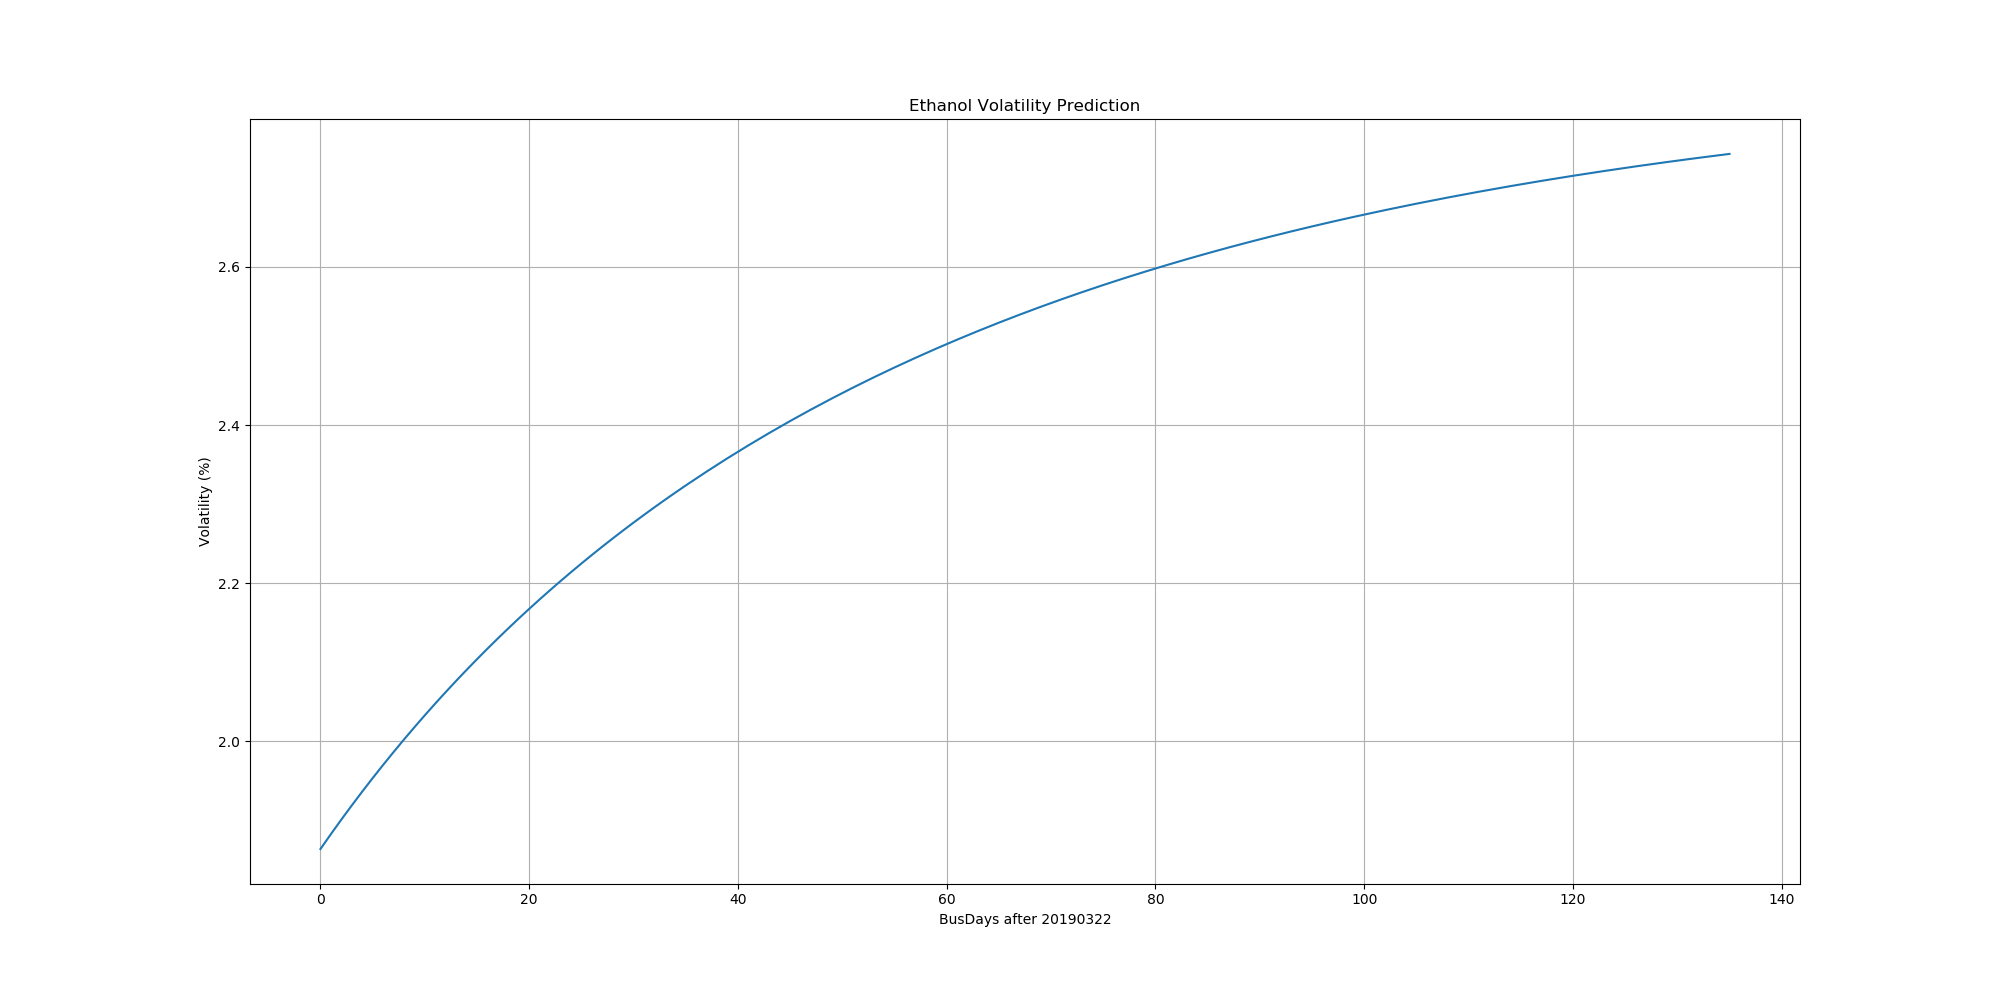
\includegraphics[width=\linewidth]{Ethanolvol.png} % Figure image
	\caption{Volatility Prediction on Ethanol} % Figure caption
	\label{eth pred} % Label for referencing with \ref{bear}
\end{figure}

\end{frame}

\begin{frame}{GJR-GARCH Model Volatility Predictions}

\begin{figure}[!ht]
	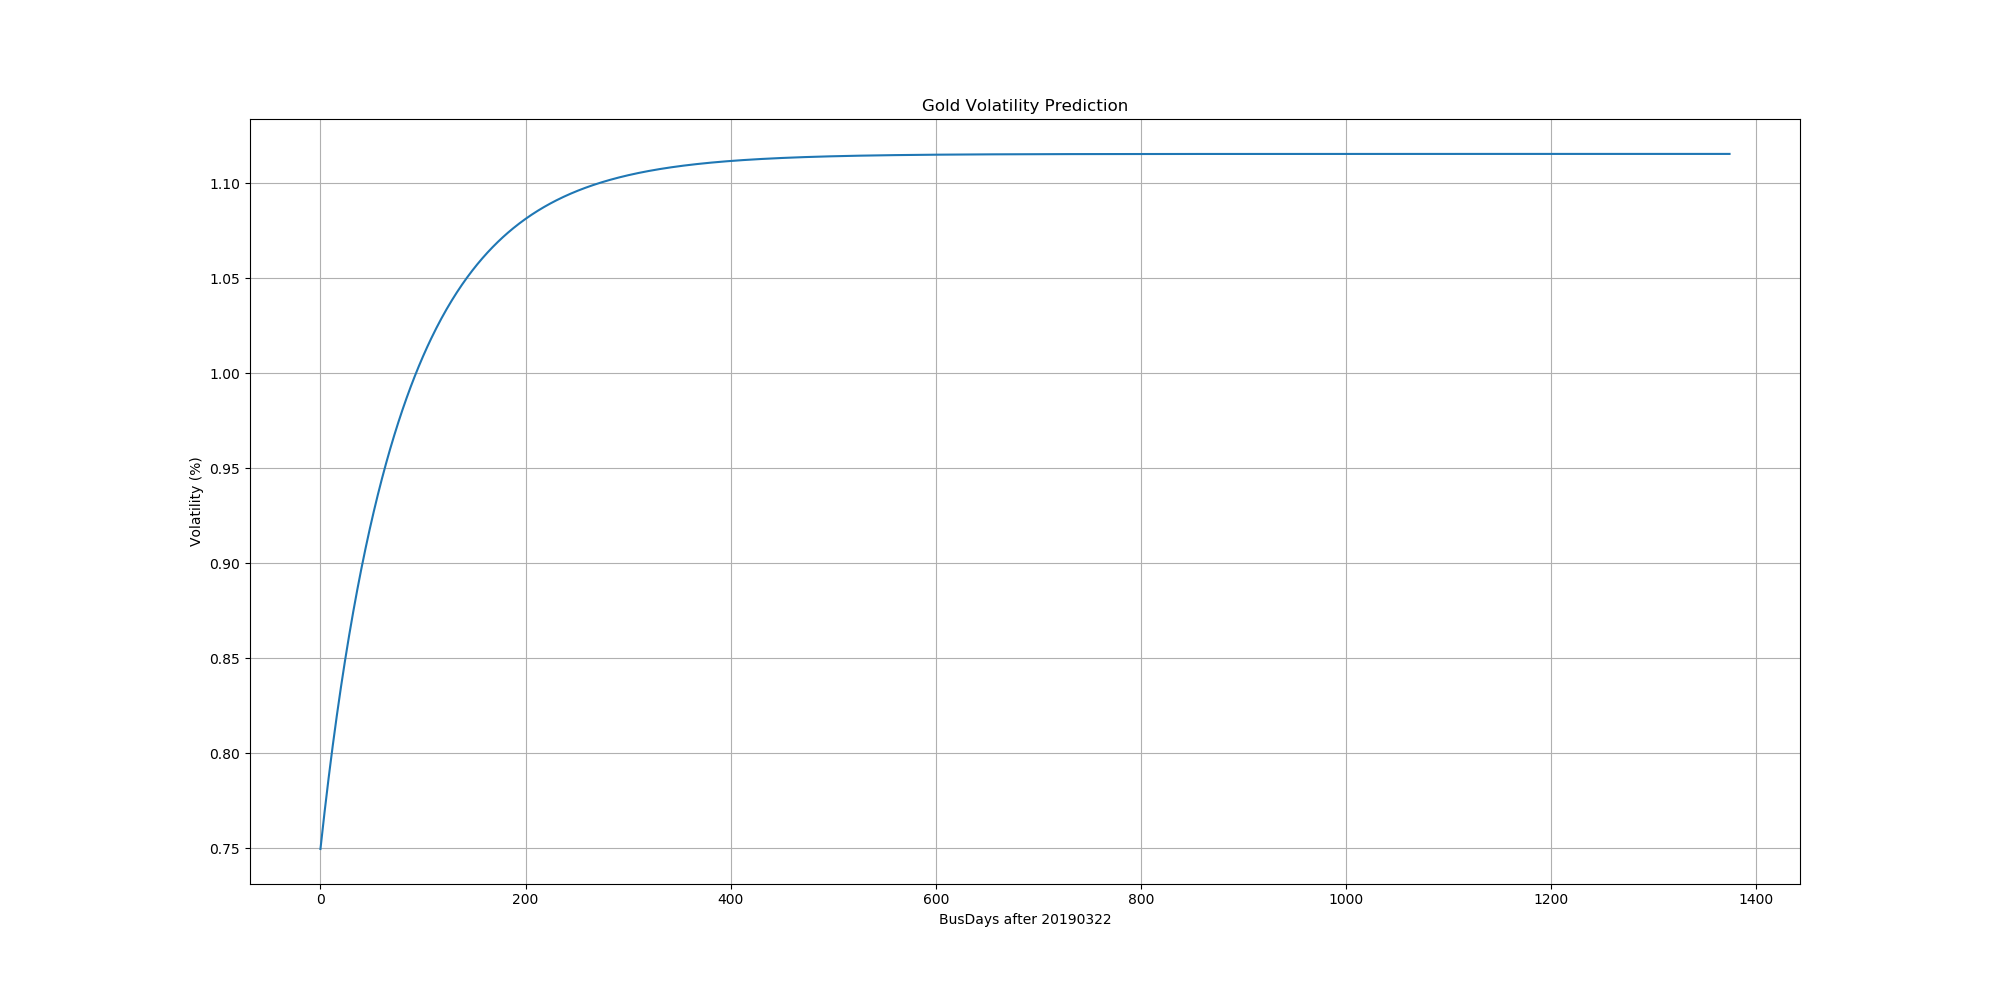
\includegraphics[width=\linewidth]{Goldvol.png} % Figure image
	\caption{Volatility Prediction on Gold} % Figure caption
	\label{gold pred} % Label for referencing with \ref{bear}
\end{figure}

\end{frame}

\begin{frame}{GJR-GARCH Model Volatility Predictions}

\begin{figure}[!ht]
	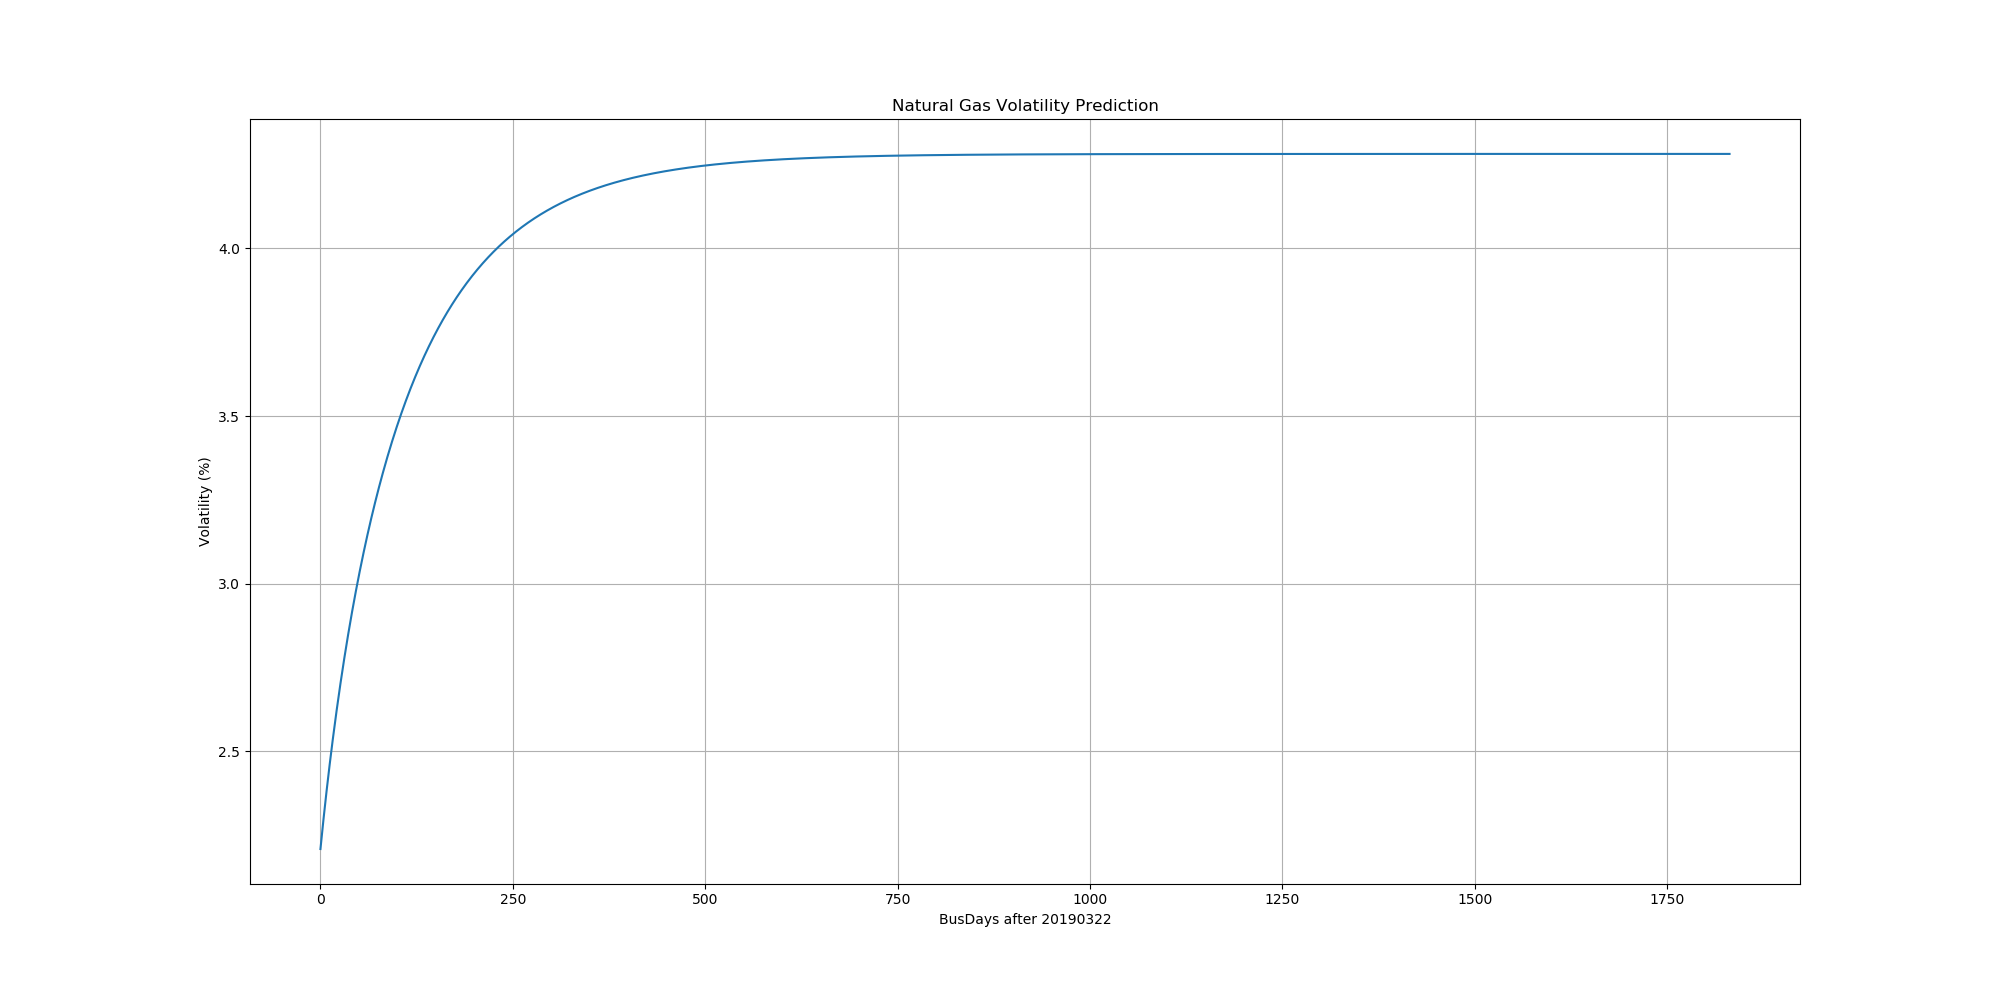
\includegraphics[width=\linewidth]{Naturalgasvol.png} % Figure image
	\caption{Volatility Prediction on Natural Gas} % Figure caption
	\label{gas pred} % Label for referencing with \ref{bear}
\end{figure}

\end{frame}

\begin{frame}{GJR-GARCH Model Volatility Predictions}

\begin{figure}[!ht]
	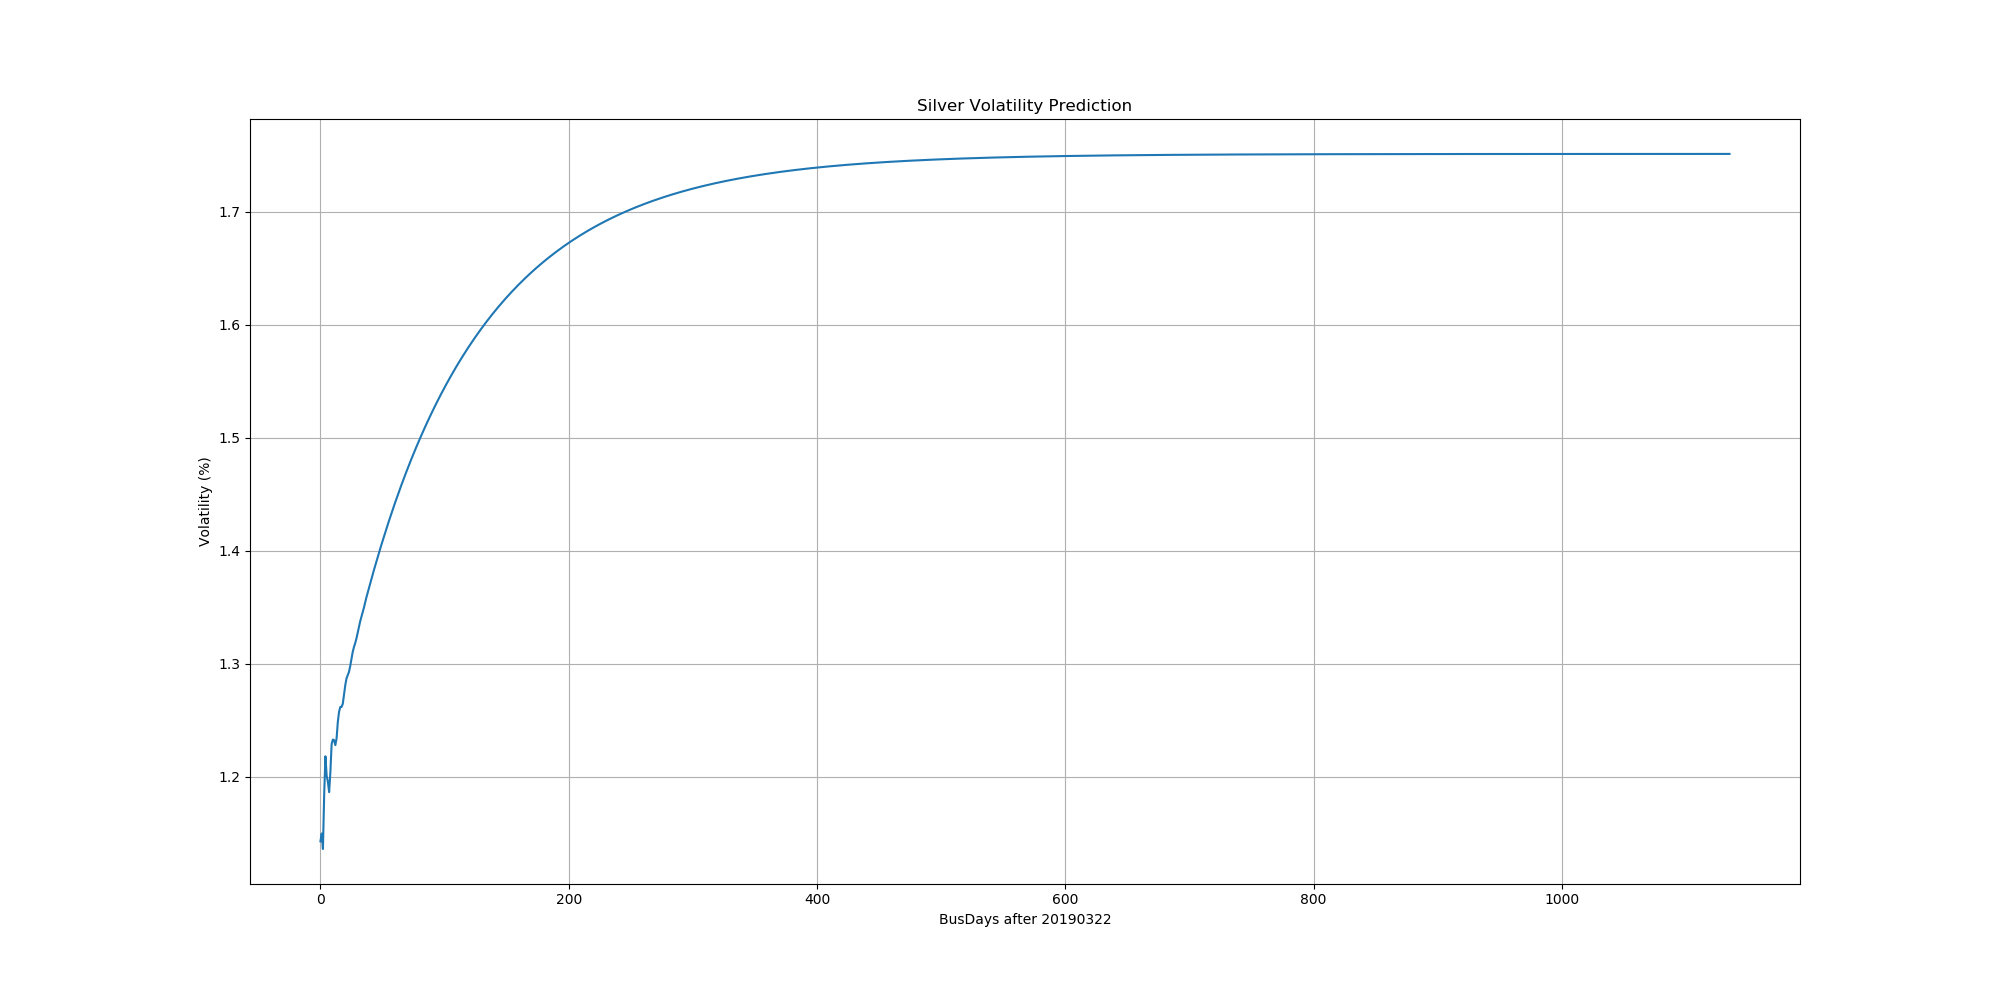
\includegraphics[width=\linewidth]{Silvervol.png} % Figure image
	\caption{Volatility Prediction on Silver} % Figure caption
	\label{silver pred} % Label for referencing with \ref{bear}
\end{figure}

\end{frame}

\begin{frame}{GJR-GARCH Model Selection Criteria}

For each commodity, the best model configuration, say the number of $\alpha$, $\beta$, $\gamma$ and whether using zero mean, is selected based on the following steps.

\begin{itemize}
	\item  Define a GJR-GARCH model: define p, o, q and fit historical with constant mean model. p, o, q are taken from 0 to 9, so there are 1000 possible models to fit.
	\item zero mean vs constant mean: if the p-value of $\mu$ in constant mean model is larger than 0.05, then the mean is considered insignificant, and it will be removed to refit the corresponding zero mean model.
	\item Ljung-Box test: the fitted model will be plugged into historical data, and the series of $\{ Z_t\}$ is derived. If $\{ Z_t\}$ passes Ljung-Box test at a significance level of 0.05, then it proves that the model well explains the historical time series. Otherwise, the model will be rejected, and go to step 1.
	\item BIC and number of parameters: if one model has a less BIC and less number of parameters than the other one, it will be selected as the temporary best model. Alternatively, if BIC of one model is $5\%$ less than the other one, it will also win the selection.
\end{itemize}

\end{frame}

\begin{frame}{Monte Carlo Simulation Scheme}
Given a commodity start price $S_0$ and a fitted GJR-GARCH model $GJR-GARCH(p,o,q)$, the underlying price movements can be simulated by the dynamics of its log returns $\{r_i\}$:

\begin{equation}
\begin{aligned}
\sigma_i &= \sqrt{\omega + \sum_{i=1}^p {\alpha_i \epsilon_{t-i}^2} + \sum_{j=1}^o {\gamma_j \epsilon_{t-j}^2 I_{\epsilon_{t-j} < 0}} + \sum_{k=1}^q {\beta_k \sigma_{t-k}^2}}
\\
Z_i &\sim N(0,1), \Delta t = 1/252
\\
\epsilon_i &= \sigma_i Z_i
\\
r_i &= \mu \Delta t + \epsilon_i
\\
S_{t_i} &=S_{t_{i-1}}\exp(r_i \Delta t) = S_0\exp(\sum_{k=0}^i r_k \Delta t)
\end{aligned}
\end{equation}
\end{frame}

\begin{frame}{Monte Carlo Simulation Scheme}
The final payoff is calculated as

\begin{equation}
\begin{aligned}
A_{t_N}(0,t_N) &= \frac 1N \sum_{i=0}^N S_{t_i}
\\
df(0,Tt_N) &= \exp (-\sum_{i=0}^{N-1} r_{t_i}\Delta t)
\\
V_{t_N} &= (A_{t_N}(0,t_N) - K)^+
\\
\bar V_{t_N} &= \frac 1n \sum_{i=1}^n V_{t_N}^i
\\
\bar V_0 &= df(0,Tt_N) \bar V_{t_N}
\end{aligned}
\end{equation}

\end{frame}

\subsection{Monte Carlo Constant Volatility Model}

\begin{frame}{Monte Carlo Constant Volatility Model}
Constant volatility model assumes that the underlying price follows the following dynamics:

\begin{equation}
\begin{aligned}
dS_t &= (r_t - \frac 12 \sigma^2)S_t dt + \sigma S_t dW_t
\\
d\log S_t &= (r_t - \frac 12 \sigma^2) dt + \sigma dW_t
\end{aligned}
\end{equation}

The constant volatility model shares the same Monte Carlo scheme with GJR-GARCH scheme, except for its path generating scheme for the underlying.

\begin{equation}
\begin{aligned}
dW_t &\sim N(0,\Delta t), \Delta t = 1/252
\\
r_i &= r_{i-1} + (r_t - \frac 12 \sigma^2) \Delta t + \sigma dW_t
\\
S_{t_i} &=S_{t_{i-1}}\exp(r_i \Delta t) = S_0\exp(\sum_{k=0}^i r_k \Delta t)
\end{aligned}
\end{equation}

The rest process follows that of GARCH scheme

\end{frame}

\subsection{Binomial Tree Model Pricing}

\begin{frame}{Binomial Tree Model for Asian Options}
\begin{itemize}
\item Forward shooting gird: approximate the average price.
\item $ S^n_j $ and $ A^n_k $: the asset value jumping upward $ j $ times and average price with index $ k $ at $ n $-th time level, respectively.

\begin{equation}
\begin{split}
&S^n_j= S_0 e^{j \Delta W}, \ \ A^n_k = S_0 e^{k \Delta Y}, \\ &\Delta W = \sigma\sqrt{\Delta t},\ \Delta Y = \rho\Delta W j, k \in\mathbb{N}
\end{split}
\end{equation}
\item $ c^n_{j, l} $: numerical approximation to the Asian call value at $ (n, j) $ node with the averaging state variable assuming the value $ A^n_l $.

\item Gird function:
\begin{equation}\label{arith: grid func}
k^{\pm}(j) = \frac{\ln\frac{(n + 1) \exp(k \Delta Y) + \exp((j \pm 1) \Delta W)}{n + 2}}{\Delta Y}
\end{equation}
\item Interpolation:
\begin{equation}\label{arith: interpolation}
c^n_{j, l} = c^n_{j, l_{floor}} + \varepsilon_l (c^n_{j, l_{ceil}} - c^n_{j, l_{floor}})
\end{equation}
where $ \varepsilon_l $ is the fraction of one step $ \Delta Y $ between $ \ln A^n_{l_{ceil}} $ and $ A^n_{l_{floor}} $:
\begin{equation}
\varepsilon_l = \frac{\ln\frac{A^n_l}{A^n_{l_{floor}}}}{\Delta Y}, A^n_l =  A^n_{l_{floor}} e^{\varepsilon_l \Delta Y}
\end{equation}
\end{itemize}
\end{frame}

\begin{frame}{Binomial Tree Model for Asian Options}
Backward induction:

\begin{equation}\label{arith: back induction}
\begin{split}
c^n_{j, k} &= \frac{1}{R} \left[ p c^{n + 1}_{j + 1, k^+(j)} + (1 - p) c^{n + 1}_{j - 1, k^-(j)}\right] \\
&\approx \frac{1}{R} \{ p \left[ \varepsilon_{k^+(j)} c^{n + 1}_{j + 1, k^+_{ceil}} + (1 - \varepsilon_{k^+(j)}) c^{n + 1}_{j + 1, k^+_{floor}} \right] \\
&+ (1 - p) \left[ \varepsilon_{k^-(j)} c^{n + 1}_{j - 1, k^-_{ceil}} + (1 - \varepsilon_{k^-(j)}) c^{n + 1}_{j - 1, k^-_{floor}} \right]\} \\
&n = N - 1, \cdots, 0, j = -n, -n + 2, \cdots, n, \\
&k \in \mathbb{N} \cap [-\frac{n}{p}, \frac{n}{p}]
\end{split} 
\end{equation}
where the risk neutral probability of jump upward is:
\begin{equation}
p=\frac{R-d}{u-d}, \ \ R = e^{r_t (T - t)}
\end{equation}
where $ r_t $ is the forward rate at time $ t $
\end{frame}

\begin{frame}{Binomial Tree Simulation}
Parameter setting:
\begin{itemize}
\item $ \sigma $: historical volatility of log return.
\item $ r_t $: forward rate at time $ t $.
\item Number of time steps $ N $:  total number of business days from the spot date to maturity date. If the time length reaches over 1 year, we restrict the time steps to 252.
\item $ \Delta t $: $ \frac{1}{N} $.
\item Underlying: 1 unit.
\end{itemize}
\end{frame}

\section{Results}

\frame{\tableofcontents[currentsection]}

\subsection{Fitted GJR-GARCH Model}

\begin{frame}{Fitted GJR-GARCH Model}
\begin{table}[!ht]
\centering
\begin{tabular}{ccccc}
\toprule
Underlying & $ (\alpha, \gamma, \beta) $ & $ Q(20) $ & p-value & BIC \\
\midrule
Crude Oil WTI & (1,1,1) & 13.69 & 0.84 & 21129 \\
Ethanol & (1,1,1) & 39.91 & 0.005 & 13715 \\
Gold & (1,0,1) & 27.53 & 0.12 & 14403  \\
Natural gas & (1,0,1) & 23.48 & 0.2 & 24608 \\
Silver & (1,0,5) & 29.42 & 0.07 & 12151 \\
\bottomrule
\end{tabular}
\caption{Model result: GJR model for each underlying futures}
\label{model result}
\end{table}
\end{frame}

\subsection{Model Pricing Results}

\begin{frame}{Model Pricing Results}
\begin{itemize}
\item ARE:
\begin{equation}\label{are}
ARE = \frac{1}{N} \sum^N_{j = 1} \frac{\vert V^{model}_j - V^{market}_j \vert}{V^{market}_j} \times 100
\end{equation}
\begin{table}
\centering
\footnotesize
\begin{tabular}{lcccccc}
\toprule
\multirow{2}{*}{Models}  & \multicolumn{2}{c}{Crude Oil WTI} & \multicolumn{2}{c}{Ethanol} & \multicolumn{2}{c}{Gold} \\
 & put & call & put & call & put & call  \\
\midrule
GARCH-MC & 46.679 & 304.798 & 10.757 & 25.258 & 72.799 & 84.586 \\ 
MC & 83.121 & 122.238 & 56.035 & 73.732 & 52.874 & 91.129 \\
BT & 402.088 & 819.106 & 45.110 & 62.466 & 106.801 & 149.124 \\
\toprule
\multirow{2}{*}{Models}  & \multicolumn{2}{c}{Silver} & \multicolumn{2}{c}{Natural gas} & & \\ & put & call & put & call  \\
\midrule
GARCH-MC & 17.455 & 26.597 & 215.232 & 324.858 \\ 
MC & 64.379 & 89.397 & 64.891 & 84.962 \\
BT & 83.969 & 107.557 & 264.242 & 72.697 \\
\bottomrule
\end{tabular}
\caption{ARE for the Asian put ans call option for each underlying futures.}
\label{are stat}
\end{table}
\item Fair price of European option: fair price of the Asian option $ < $ the European option value with the same specification of options: all average option values from 3 models $  <  $ European option value with the same specification
\end{itemize}
\end{frame}

\section{Discussions}

\frame{\tableofcontents[currentsection]}

\begin{frame}{Discussions}
\begin{itemize}
	\item Data Limitations: lack of underlying price and option information. 
	\begin{itemize}
		\item Using future prices rather than spot prices to fit models. 
		\item Only WTI Crude Oil Asian Option price and Chicago Ethanol (Platts) Asian Option are Asian options.
	\end{itemize}

	\item Monte Carlo Limitations standard deviation of simulated payoffs is relatively large.
	\begin{itemize}
		\item The number of simulated paths might not be enough: increase the number of paths.
		\item Apply probability bounds analysis (PBA) to estimate upper and lower bounds of simulated payoffs.
	\end{itemize}
	\item Advanced GARCH Models\cite{lorenzo2011pricing}: semi-analytical formula for geometric Asian options
	\begin{equation}
	\begin{aligned}
	r_t &= r - \frac 12 \sigma_t^2 + \sigma_t Z_t
	\\
	\sigma_t^2 &= \omega + \alpha_1 (Z_{t-1} -\lambda \sigma_{t-1})^2+\beta_1 \sigma_{t-1}^2
	\end{aligned}
	\end{equation}
\end{itemize}
\end{frame}

\section{Conclusions}

\frame{\tableofcontents[currentsection]}

\begin{frame}{Conclusions}

\begin{itemize}
	\item 16 commodity future prices are studied.
	\item 5 options are priced by three pricing methods, say binomial tree model, Monte Carlo simulations with constant volatility, and Monte Carlo simulations with GJR-GARCH volatility.
	\item Strong sector correlations are discovered in the 16 time series of commodity log returns.
	\item The ARE criterion shows that GJR-GARCH model is the most appropriate pricing model in three models.
	\item Limitations in data and models can be overcomed in future studies.
\end{itemize}

\end{frame}

\begin{frame}[allowframebreaks]{References}
\bibliographystyle{unsrt}
\bibliography{example.bib}
\end{frame}


\end{document}

